\documentclass{article}

\usepackage[dvips]{graphicx}

\usepackage{natbib}
\bibliographystyle{apa}

\usepackage{url}

\newenvironment{eqnnon}{\begin{equation}}{\end{equation}}
\newenvironment{eqnarraynon}{\begin{eqnarray}}{\end{eqnarray}}

\newcommand{\mat}{A}
\newcommand{\sol}{b}
\newcommand{\eqmat}{F}
\newcommand{\eqvec}{h}
\newcommand{\ineqmat}{G}
\newcommand{\ineqvec}{k}

\newcommand{\cost}{c}
\newcommand{\eqfn}{f}
\newcommand{\ineqfn}{g}

\newcommand{\coord}{x}

\newcommand{\matEl}{a}
\newcommand{\eqmatEl}{f}
\newcommand{\inveqsubmat}{R}
\newcommand{\inveqsubmatEl}{r}
%doesn't work:
%\newcommand{\element}[1]{\lowercase{#1}}

\newcommand{\slack}{\mu}

\title{Solving constrained least squares problems}

\begin{document}

\tableofcontents

\section{Introduction}

We are interested in solving constrained least squares problems of 
the following form:
\begin{equation}
	\min_{\vec \coord} | \mat \vec \coord - \vec \sol |
	\label{least_squares}
\end{equation}
subject to both equality constraints:
\begin{equation}
	\eqmat \vec \coord = \vec \eqvec 
\end{equation}
and inequality constraints:
\begin{equation}
	\ineqmat \vec \coord \ge \vec \ineqvec
	\label{inequality}
\end{equation}
Such problems are ubiquitous in machine learning applications.
Examples include the support vector machine dual problem, solving
for multi-class probabilities, and local approximations for iterative 
``global'' nonlinear optimizers.
This short summary discusses methods of tackling these types of problems.

\section{Equality constraints}

An intuitive method of enforcing equality constraints is through a reduction
of variables by defining some of the variables in terms of the others based
on the constraints.
If $\eqmat$ is an $m_e \times n$ matrix, then we divide it into two sub-matrices,
a square one, which we take the inverse of:
\begin{equation}
	\inveqsubmat^{-1} = \lbrace \eqmatEl_{ij} | i \in [1, m_e]; j \in [1, m_e] \rbrace
\end{equation}
and whatever is left, $\lbrace \eqmatEl_{ij} | i \in [1, m_e]; j \in [1, n-m_e] \rbrace$.
We solve the first $m_e$ of the variables in terms of the remaining $n-m_e$ variables:
\begin{equation}
	\coord_i=\sum_{j=1}^{m_e} \inveqsubmatEl_{ij} \left ( \eqvec_j - \sum_{k=m_e}^n \eqmatEl_{jk} \coord_k \right ) | i =[1..m_e]
\end{equation}
To solve the problem, we substitute this into the unconstrained least-squares
problem in (\ref{least_squares}):
\begin{equation}
	\min_{\lbrace x_i|i \in [m_e, n] \rbrace} \sum_{i=1}^n \left [ \sum_{j=m_e}^n \matEl_{ij} \coord_j + \sum_{j=1}^{m_e} \matEl_{ij} \sum_{k=1}^{m_e} \inveqsubmatEl_{jk} \left ( \eqvec_k - \sum_{l=m_e}^n \eqmatEl_{kl} \coord_l \right ) - \sol_i \right ]^2
\end{equation}
Rearranging the summation order and gathering the constant terms:
\begin{equation}
	\min_{\lbrace x_i|i \in [m_e, n] \rbrace} \sum_{i=1}^n \left [ \sum_{j=m_e}^n \left ( \matEl_{ij} + \sum_{k=1}^{m_e} \matEl_{ik} \sum_{l=1}^{m_e} \inveqsubmatEl_{kl} \eqmatEl_{lj} \right ) \coord_j 
	- \sol_i + \sum_{j=1}^{m_e} \matEl_{ij} \sum_{k=1}^{m_e} \inveqsubmatEl_{jk} \eqvec_k \right ]^2
\end{equation}
	
\section{Lagrange multipliers}

A more symmetric method of enforcing equality constraints is through Lagrange
multipliers.
This actually increases the number of variables but the number of new variables
is equal to the number of constraints, thus the problem remains well-posed.

Let $\cost$ be a (nonlinear) function to be minimized and let $\lbrace \eqfn_i \rbrace$ be a set of functions describing equality constraints:
\begin{equation}
	\eqfn_i(\vec \coord) = 0
 	\label{equality2}
\end{equation}
We can use a Lagrange multiplier to add the constraint to the optimization
problem:
\begin{equation}
	\min_{\lbrace \vec \coord, \vec \lambda \rbrace} \left \lbrace \cost(\vec \coord) + \sum_i \lambda_i \eqfn_i(\vec \coord) \right \rbrace
\end{equation}
where $\vec \lambda=\lbrace \lambda_i \rbrace$ are a set of {\it Lagrange multipliers}.
Taking the gradient and setting it to zero:
\begin{equation}
	\nabla_{\vec \coord} \cost + \sum_i \lambda_i \nabla_{\vec \coord} \eqfn_i = 0 
	\label{lagrange2}
\end{equation}
Note that taking the derivative with respect to the Lagrange multiplier
returns the equality constraint in (\ref{equality2}).
For the least squares problem in (\ref{least_squares}), 
Equation (\ref{lagrange2}) reduces to:
\begin{equation}
	\mat^T \mat \vec \coord + \vec \lambda \eqmat = \mat^T \vec \sol
\end{equation}
\citep{Lawson_Hanson1995}

\begin{figure}
	\includegraphics[width=0.9\textwidth]{Lagrange.eps}
	\caption{Illustration of Lagrange multiplier technique for equality constraints.}
\end{figure}

\section{Inequality constraints}

\begin{figure}
	\includegraphics[width=0.9\textwidth]{inequality.eps}
	\caption{Illustration of an inequality constraint.}\label{ineq_fig}
\end{figure}

With a slight variation, Lagrange multipliers can work with inequality
constraints.
Given a set of inequality constraints on cost function, $\cost$:
\begin{equation}
	\ineqfn_i(\vec \coord) \ge 0
 	\label{inequality2}
\end{equation}
we have:
\begin{equation}
	\nabla_{\vec \coord} \cost = \sum_i \slack_i \nabla_{\vec \coord} \ineqfn_i
\end{equation}
where the variables which take the place of the Lagrange multipliers,
now called ``slack'' variables, are themselves constrained:
\begin{equation}
	\slack_i \ge 0
\end{equation}
Note that:
\begin{eqnarray}
\slack_i = 0 & \iff & \ineqfn_i > 0 \\
	\slack_i > 0 & \iff & \ineqfn_i = 0
\end{eqnarray}
In other words, if the solution lies outside the constraint, then the slack
variable is zero because it is not needed, 
while if the solution lies on the border of the constraint,
then the slack variable is non-zero and acts as a Lagrange multiplier.
An attempt is made to illustrate this situation in Figure \ref{ineq_fig}.

Put more succinctly:
\begin{equation}
	\slack_i \ineqfn_i = 0
\end{equation}


\bibliography{../ML_learning}

\end{document}


